Este capítulo apresenta a elaboração teórica da dinâmica do drone híbrido em modo multirrotor. Sob a hipótese de corpo rígido, detalham-se as equações não lineares dos modelos rotacional e translacional, que descrevem o voo com seis graus de liberdade (6-DOF). Introduzem-se ainda a nomenclatura e os sistemas de coordenadas utilizados na formulação matemática, as equações cinemáticas de atitude e de posição e o modelo dos motores com a respectiva alocação de controle. A linearização desse modelo em torno do voo pairado, utilizada no projeto de controle, é apresentada no Apêndice~\ref{ap:linearizacao}.


\section{Sistemas de Coordenadas}

Para o estudo e representação de \gls{MAV}, é importante compreender as diferentes formas de observar os objetos em movimentos, pois cada sistema de coordenadas utiliza um referencial diferente para representação da cinemática do corpo nas acelerações, velocidades, posições, e também da sua dinâmica através das forças e momentos aplicados \cite{Farrell2008}. Quanto à notação, grandezas vetoriais, vetores-coluna e matrizes são grafados em negrito, enquanto módulos e componentes escalares aparecem em itálico simples, e os eixos dos referenciais são indicados por seus rótulos, como $i^b$, $j^b$ e $k^b$. Estes sistemas são apresentados a seguir:

\subsection{Referencial de Navegação Local}

Um dos principais sistemas de coordenadas é baseado no referencial de navegação local, fixado em um ponto na superfície da Terra, conforme apresenta a Figura \ref{navigation-frame}. Levando em consideração o pequeno porte e as distâncias percorridas pelo MAV, as variações decorrentes do formato da Terra podem ser simplificadas para um plano tangente \cite{Farrell2008}. A posição é dada na referência \gls{NED}, determinada por $\mathbf{p}^{g}=[x,y,h]$, em que:

\begin{itemize}
    \item $x$: posição ao longo do eixo $i^i$, que aponta para o norte;
    \item $y$: posição ao longo do eixo $j^i$, que aponta para o leste;
    \item $h$: altitude na direção do eixo $k^i$, que aponta para o centro da Terra.
\end{itemize}

\begin{figure}[ht]
  \centering
  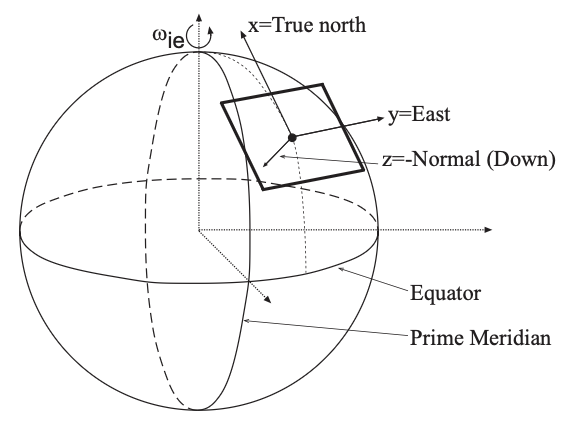
\includegraphics[width=0.45\textwidth]{Cap2/NAVIGATION-FRAME.png}
  \caption{Plano tangente de Navegação Local \cite{Farrell2008}.}
  \label{navigation-frame}
\end{figure}

A velocidade do corpo é dada por $\mathbf{v}^{g} = [v_n,v_e,v_d]$, e representa o movimento em $m/s$ ao longo dos eixos citados acima. Estas definições são importantes porque a trajetória do objeto em relação à Terra é determinada por este sistema de coordenadas. Por isso, um controlador de altitude e de velocidade vertical precisa estar baseado neste referencial. Além disso, para facilitar a compreensão da seção seguinte, adota-se o referencial de navegação projetado no drone, com origem no centro de gravidade: o eixo $i^v$ aponta para o norte, o eixo $j^v$ aponta para o leste e o eixo $k^v$ aponta para o centro da Terra. A Figura \ref{navigation} compara estes dois sistemas de coordenadas de navegação e veículo \cite{Beard2012}.

\begin{figure}[ht]
  \centering
  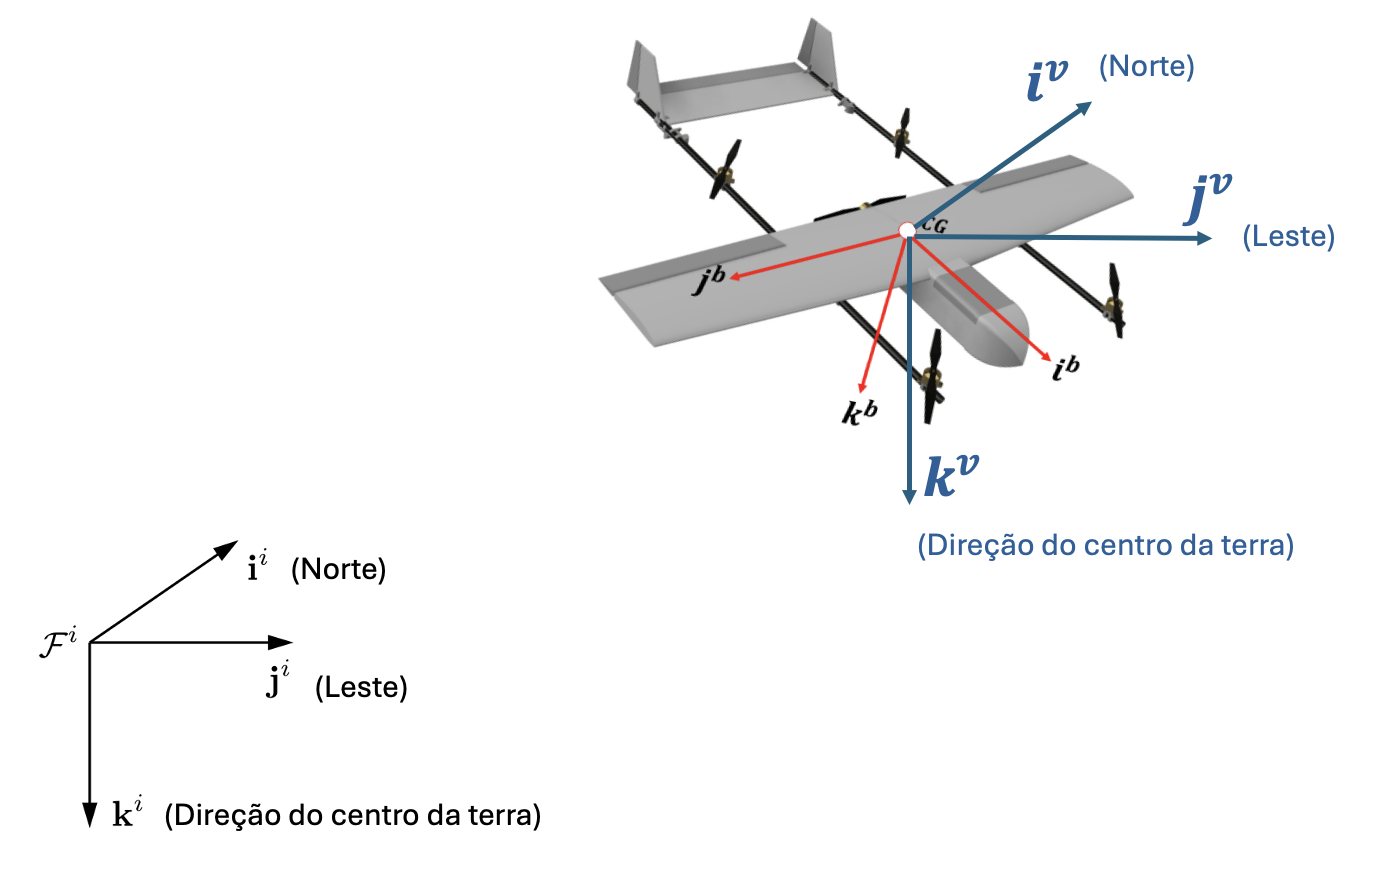
\includegraphics[width=0.9\textwidth]{Cap2/NAV.png}
  \caption{Referencial de Navegação local, fixo à superfície da Terra e sistema de coordenadas do corpo, fixo ao CG da aeronave \cite[Adaptado de][]{Beard2012}.}
  \label{navigation}
\end{figure}

\subsection{Referencial do Corpo}

Apesar do sistema controlador de altitude se basear no referêncial de navegação, existem alguns sensores que são incorporados e fixados no MAV, como acelerômetros e giróscópios, que possuem uma resposta inercial em relação ao centro de gravidade do drone (CG), nos eixos $i^b$ que aponta para a frente do drone, $j^b$ que aponta para asa direita e $k^b$ que aponta para a base do drone, medindo suas forças específicas e velocidades angulares, conforme apresenta a Figura \ref{body-frame} \cite{Beard2012}.

\begin{figure}[ht]
  \centering
  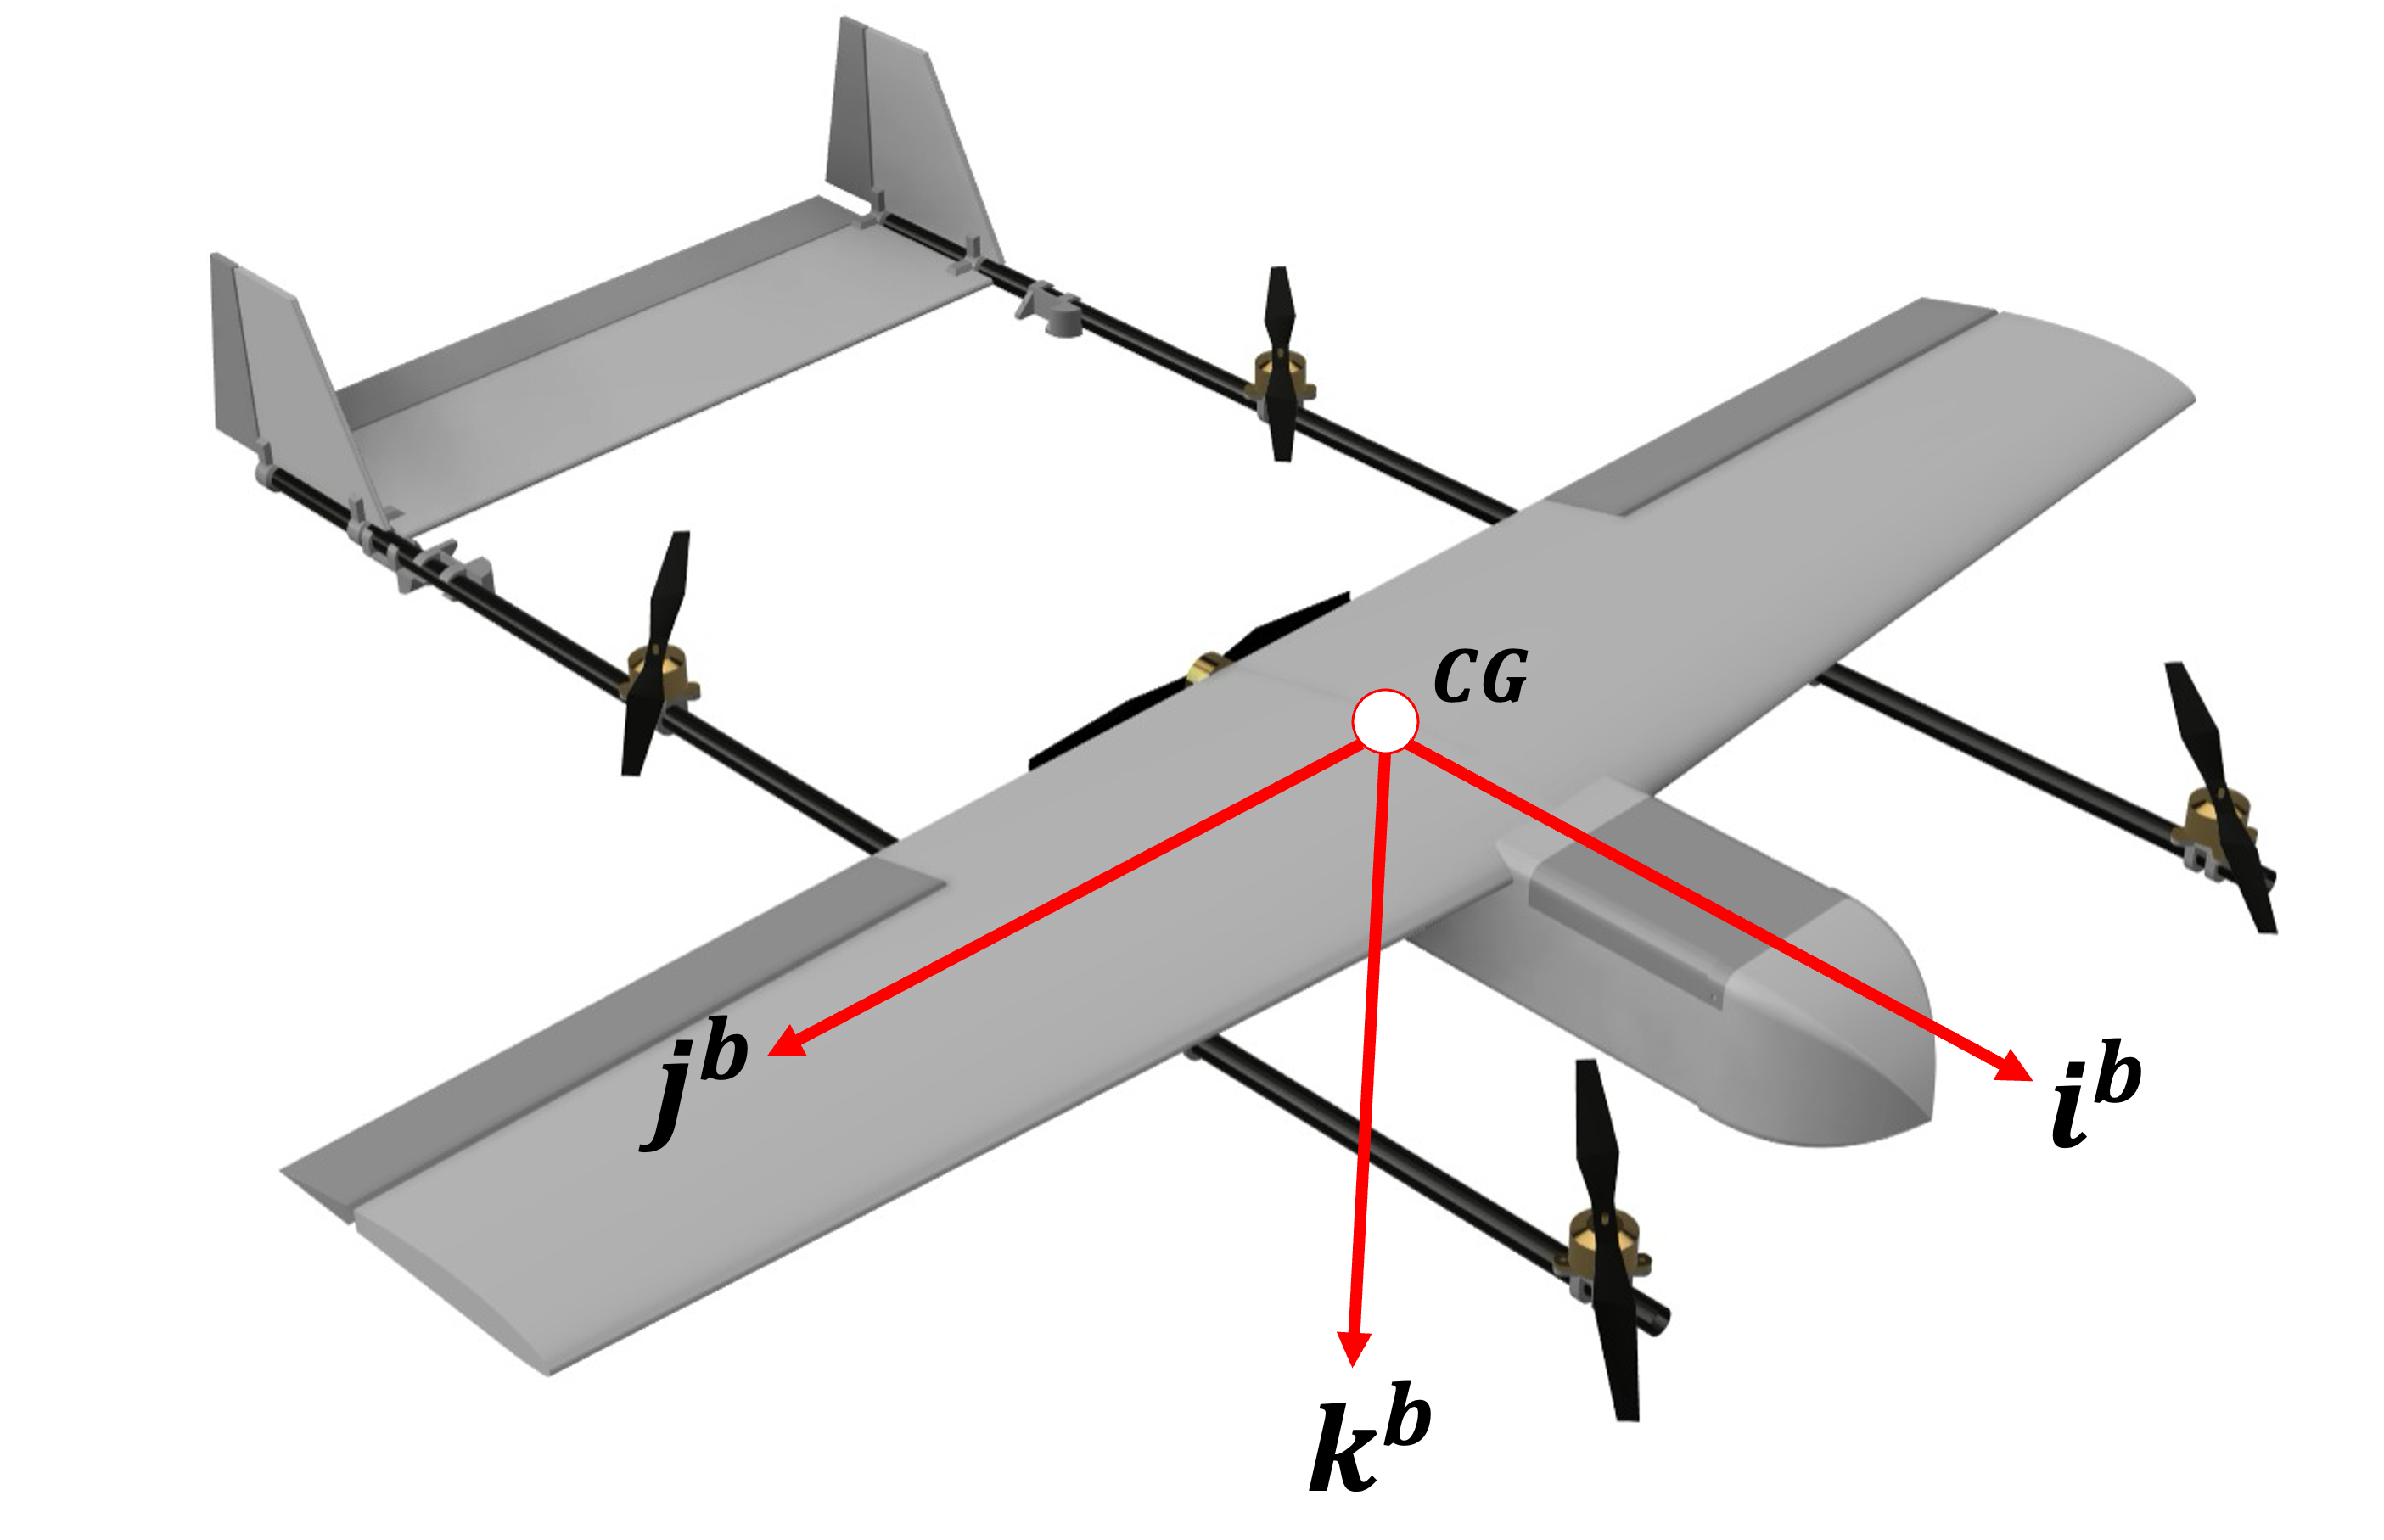
\includegraphics[width=0.5\textwidth]{Cap2/BODY-FRAME.png}
  \caption{Referencial do Corpo no Drone Híbrido (Criado pelo próprio autor).}
  \label{body-frame}
\end{figure}

A velocidade angular, no referencial do corpo, é dada por $\boldsymbol{\omega}^{b} = [p,\,q,\,r]$, enquanto a velocidade linear do corpo é representada por $\mathbf{v}^{b} = [u,v,w]$, os quais são as principais variáveis para o equacionamento do modelo rotacional e translacional do drone híbrido \cite{Farrell2008}.


\section{Transformação de coordenadas}

Como os sensores inerciais, como acelerômetro e giroscópio, medem grandezas no referencial do corpo, enquanto a navegação e o controle de trajetória são descritos no referencial de navegação, é necessário relacionar vetores entre os dois sistemas. Essa relação é obtida por uma matriz de rotação $\mathbf{R}$, também chamada de matriz de cossenos diretores, construída a partir dos ângulos de Euler segundo a sequência aeronáutica padrão $3$--$2$--$1$ (guinada, arfagem e rolagem). A sequência parte do referencial de navegação e atravessa dois referenciais intermediários, $\mathcal{F}^{v1}$ e $\mathcal{F}^{v2}$, até alcançar o referencial do corpo, conforme ilustra a Figura~\ref{fig:angulos-euler} \cite{Beard2012}.

\begin{figure}[ht]
  \centering
  \subfloat[Guinada $\psi$]{%
    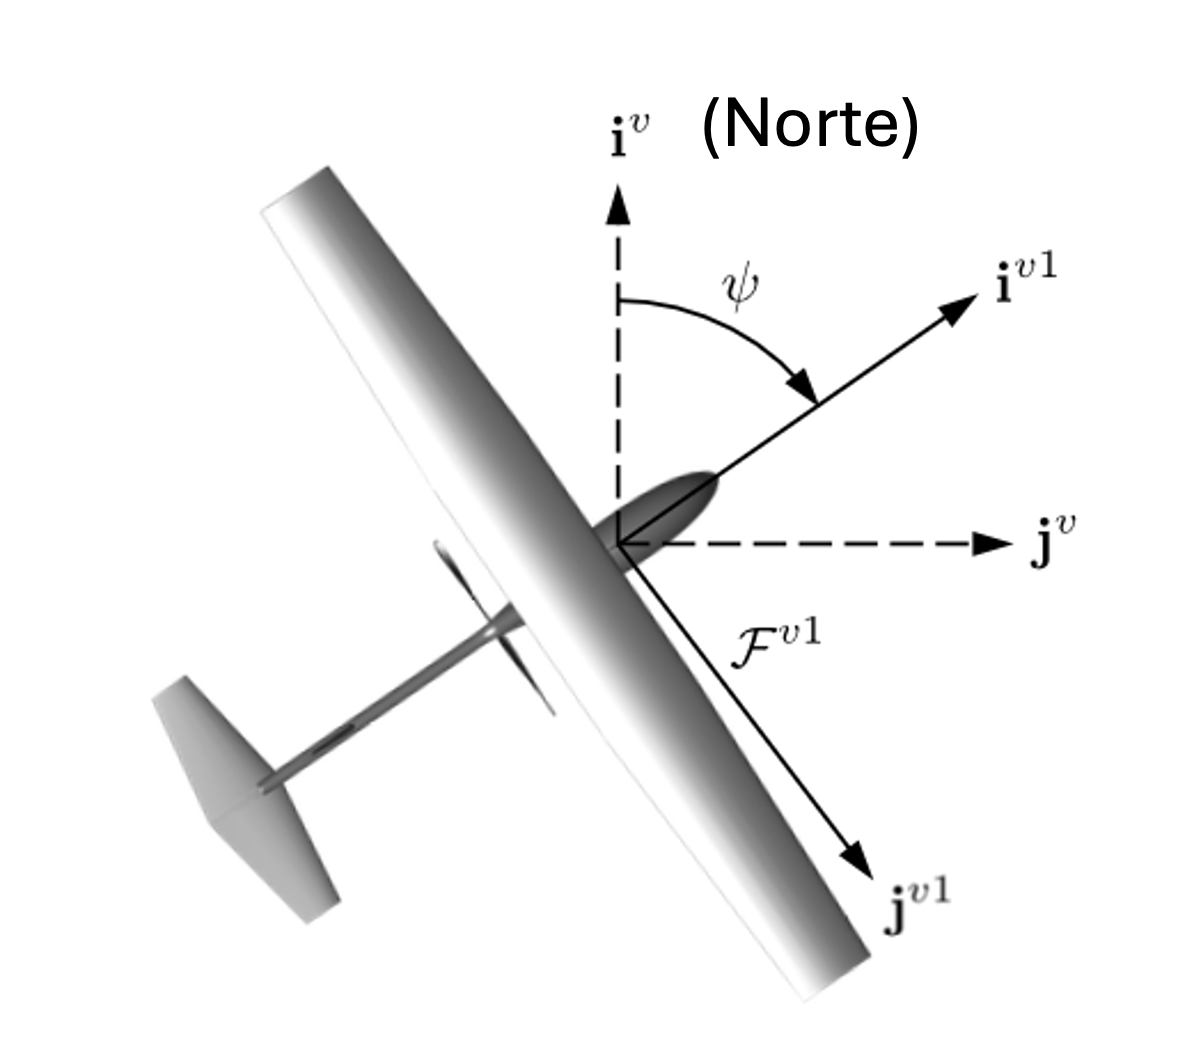
\includegraphics[width=0.25\textwidth]{Cap2/GUINADA.png}%
    \label{fig:yaw}}
  \hfill
  \subfloat[Arfagem $\theta$]{%
    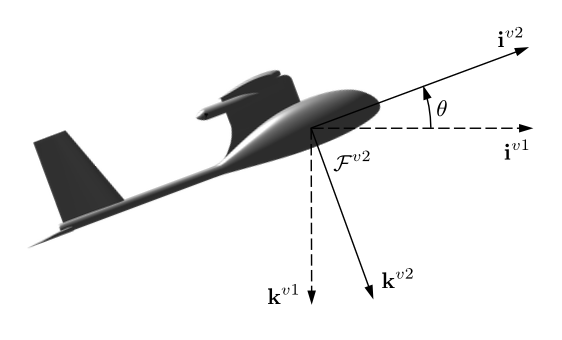
\includegraphics[width=0.33\textwidth]{Cap2/ARFAGEM.png}%
    \label{fig:pitch}}
  \hfill
  \subfloat[Rolagem $\phi$]{%
    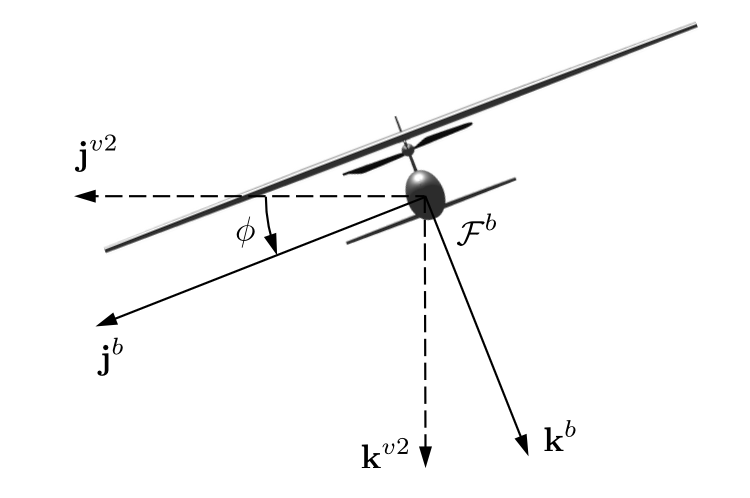
\includegraphics[width=0.33\textwidth]{Cap2/ROLAGEM.png}%
    \label{fig:roll}}
  \caption{Ângulos de Euler \cite[Adaptado de][]{Beard2012}.}
  \label{fig:angulos-euler}
\end{figure}

As três rotações elementares são aplicadas em sequência, cada uma em torno de um eixo do referencial obtido na etapa anterior: a guinada $\psi$, em torno de $k^v$, leva do referencial de navegação projetado no drone $\mathcal{F}^{v}$ ao intermediário $\mathcal{F}^{v1}$, a arfagem $\theta$, em torno de $j^{v1}$, leva de $\mathcal{F}^{v1}$ a $\mathcal{F}^{v2}$, e a rolagem $\phi$, em torno de $i^{v2} \equiv i^{b}$, leva de $\mathcal{F}^{v2}$ ao referencial do corpo $\mathcal{F}^{b}$. A matriz que leva um vetor do referencial do corpo para o de navegação resulta da composição dessas três rotações elementares:
\begin{equation}
  \mathbf{R}^{g}_{b} = \mathbf{R}_z(\psi)\,\mathbf{R}_y(\theta)\,\mathbf{R}_x(\phi),
  \label{eq:R-composicao}
\end{equation}
\begin{equation}
  \mathbf{R}_z(\psi) =
  \begin{bmatrix}
    c_\psi & -s_\psi & 0 \\
    s_\psi & \phantom{-}c_\psi & 0 \\
    0 & 0 & 1
  \end{bmatrix}\!,\quad
  \mathbf{R}_y(\theta) =
  \begin{bmatrix}
    \phantom{-}c_\theta & 0 & s_\theta \\
    0 & 1 & 0 \\
    -s_\theta & 0 & c_\theta
  \end{bmatrix}\!,\quad
  \mathbf{R}_x(\phi) =
  \begin{bmatrix}
    1 & 0 & 0 \\
    0 & c_\phi & -s_\phi \\
    0 & s_\phi & \phantom{-}c_\phi
  \end{bmatrix}\!.
  \label{eq:R-elementares}
\end{equation}

Efetuando o produto da Equação~\eqref{eq:R-composicao}, obtém-se a matriz de transformação do corpo para a navegação na forma expandida \cite{Farrell2008}:
\begin{equation}
  \mathbf{R}^{g}_{b} =
  \begin{bmatrix}
    c_\theta c_\psi & s_\phi s_\theta c_\psi - c_\phi s_\psi & c_\phi s_\theta c_\psi + s_\phi s_\psi \\[2pt]
    c_\theta s_\psi & s_\phi s_\theta s_\psi + c_\phi c_\psi & c_\phi s_\theta s_\psi - s_\phi c_\psi \\[2pt]
    -s_\theta & s_\phi c_\theta & c_\phi c_\theta
  \end{bmatrix}\!.
  \label{eq:R-corpo-nav}
\end{equation}
Assim, um vetor expresso no referencial do corpo é levado ao referencial de navegação pela multiplicação por $\mathbf{R}^{g}_{b}$, em particular, a velocidade linear satisfaz $\mathbf{v}^{g} = \mathbf{R}^{g}_{b}\,\mathbf{v}^{b}$. Por ser uma matriz ortonormal, a transformação inversa, do referencial de navegação para o do corpo, é simplesmente a sua transposta:
\begin{equation}
  \mathbf{R}^{b}_{g} = \left(\mathbf{R}^{g}_{b}\right)^{\!\top}.
  \label{eq:R-inversa}
\end{equation}
Essa propriedade é útil para projetar a aceleração da gravidade, conhecida no referencial de navegação como $\mathbf{g}^{g} = [\,0,\ 0,\ g\,]^{\top}$, sobre os eixos do corpo, etapa necessária para formular o modelo translacional e compensação das medidas de acelerômetros, retirando as parcelas devidas à gravidade, ficando apenas as acelerações devido ao movimento do corpo, como usado na próxima seção.

\begin{equation}
  \mathbf{g}^{b} = \left(\mathbf{R}^{g}_{b}\right)^{\!\top} \mathbf{g}^{g}
  = \begin{bmatrix} -\,g\,s_\theta \\ g\,s_\phi c_\theta \\ g\,c_\phi c_\theta \end{bmatrix}\!.
  \label{eq:g-corpo}
\end{equation}

\section{Equações de Movimento e Modelagem}

Para realizar a formulação das equações de movimento do drone VTOL utilizado neste trabalho, é necessário compreender que a plataforma possui uma fuselagem semelhante a um MAV asa fixa apresentado por \textcite{Beard2012}, porém, são adicionados 4 motores brushless em formato H para atuação em modo multirrotor, o qual será detalhado no capítulo seguinte. 

Assume-se que o corpo é rígido, portanto, a dinâmica ocorre a partir da relação dos momentos e empuxos gerados por esses atuadores \cite{Graesdal2021}, detalhados na Figura \ref{force-moment}.

\begin{figure}[ht]
  \centering
  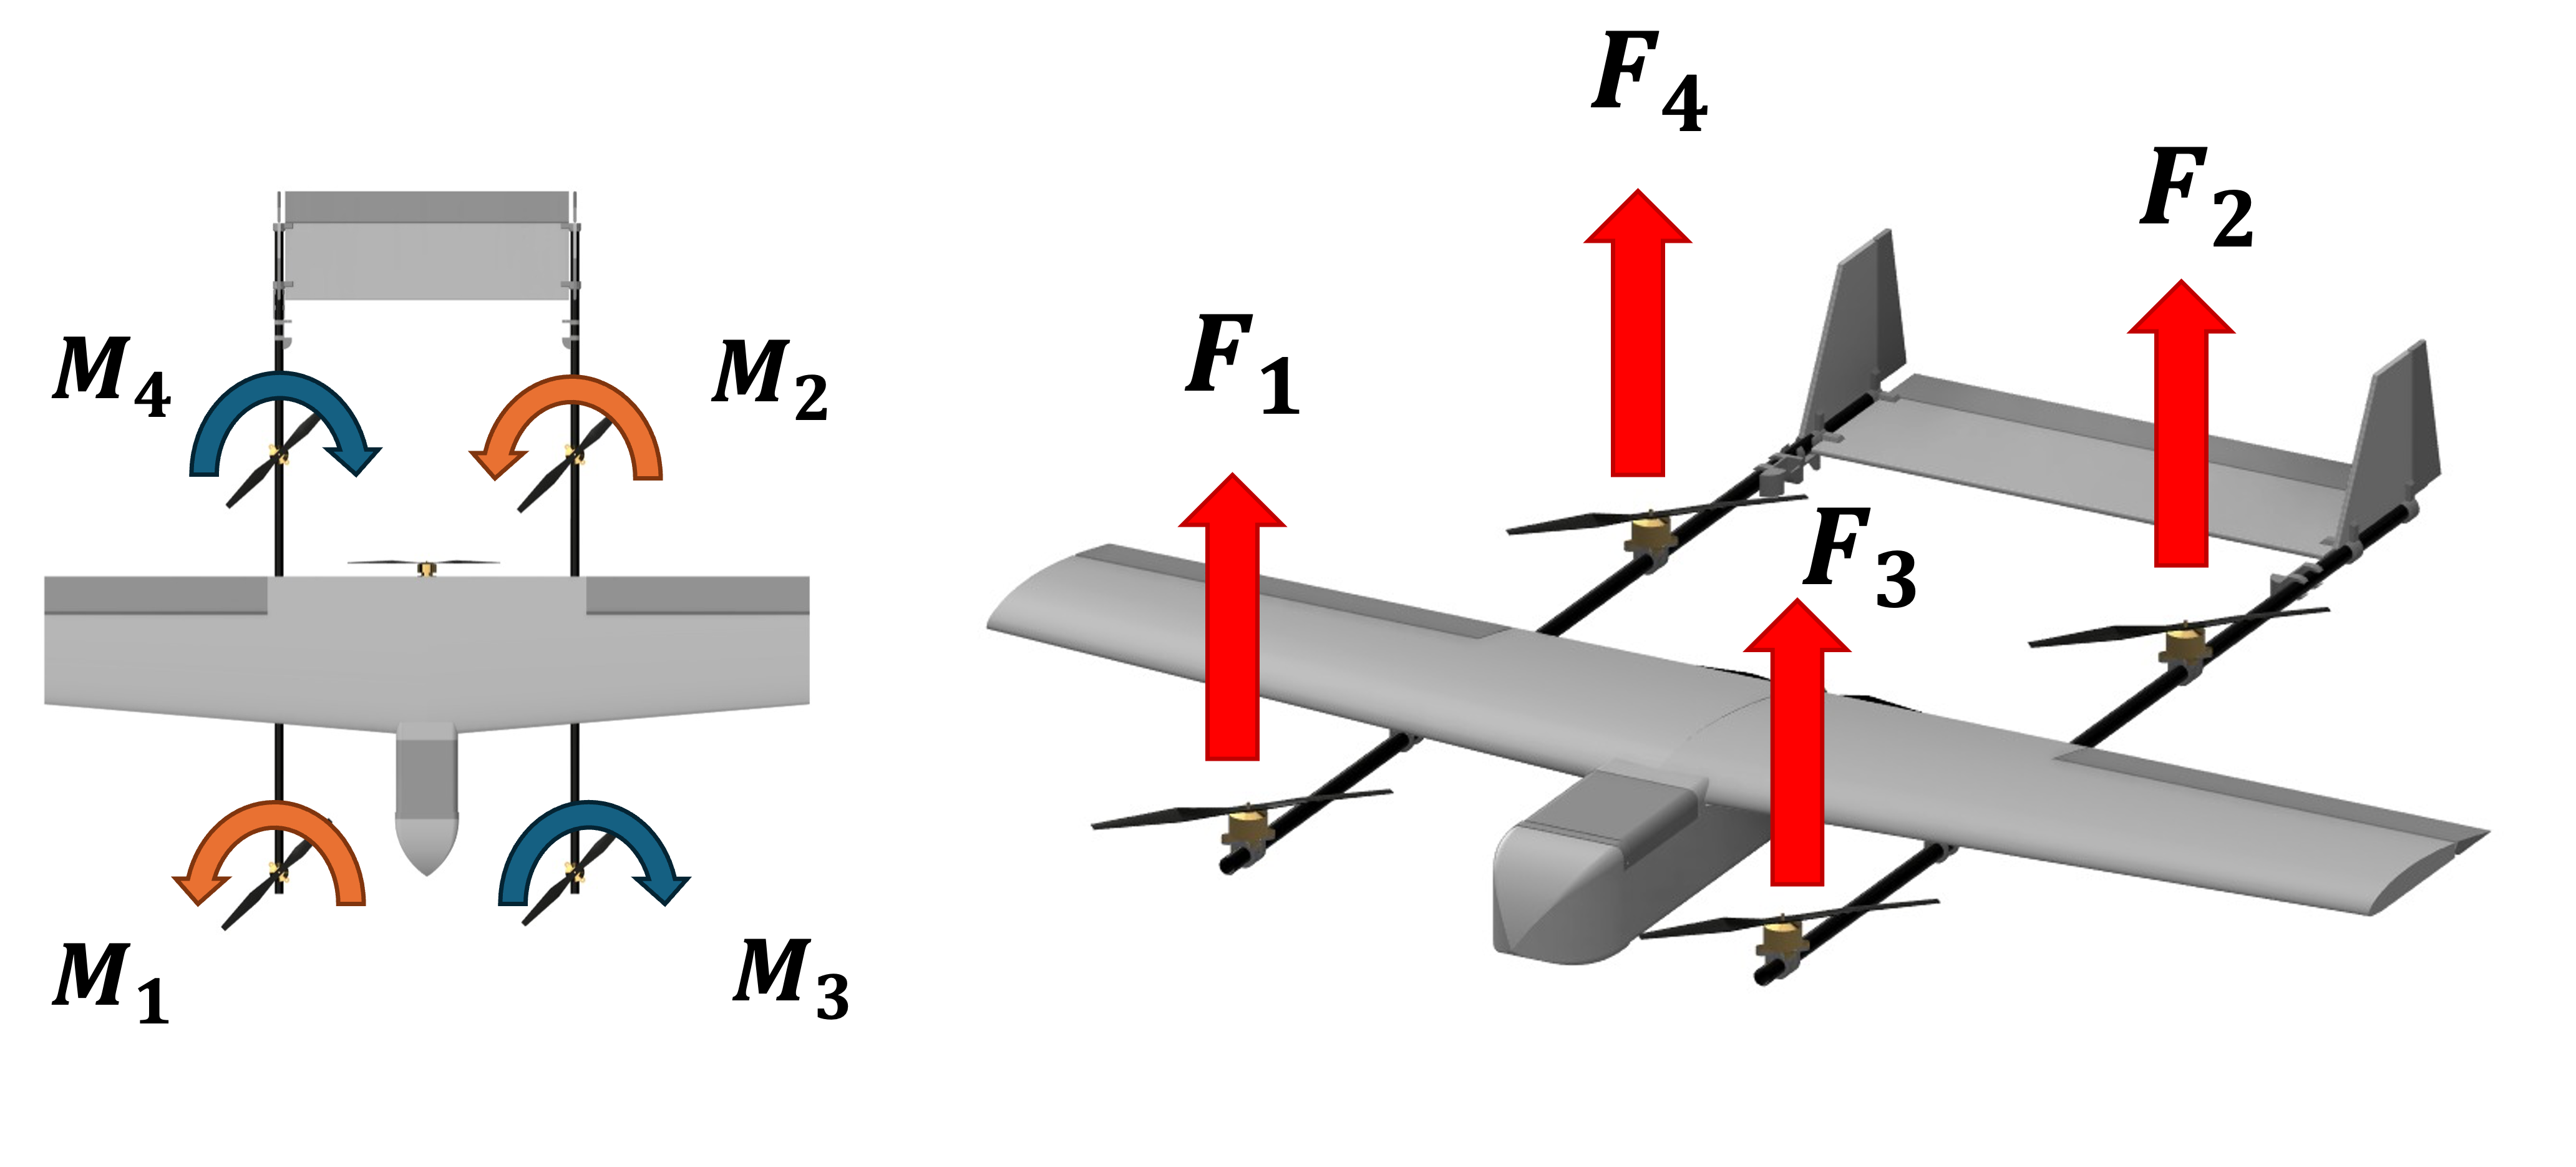
\includegraphics[width=1\textwidth]{Cap2/F-M.png}
  \caption{Relação de momentos e forças aplicados pelos motores (Criado pelo próprio autor).}
  \label{force-moment}
\end{figure}

Segundo \textcite{Quan2017}, destacado na Figura \ref{motor-model}, o sistema do multirrotor é dividido em 4 submodelos:

\begin{enumerate}
  \item \textbf{Modelo de Propulsão:} é o modelo que compõe toda a parte do mecanismo de alimentação de energia pela bateria, aplicada no motor brushless (DC) através do \gls{ESC}. Na prática, o modelo converte um comando de entrada do microcontrolador de PWM, geralmente entre $1000\mu s$ e $2000\mu s$, normalizado de 0 a 1, em velocidade angular do motor.

  \item \textbf{Alocação dos Motores:} A partir da velocidade angular desses motores, acoplados a uma hélice, é gerado um empuxo de saída em Newtons (N) e um torque de reação em (Nm), dependendo da geometria e distâncias do CG, resultam em um efeito agregado no corpo rígido do drone híbrido.
  
  \item \textbf{Modelo dinâmico:} Essas forças e momentos gerados pelos motores realizam movimento de rotação e translação no corpo rígido, resultando nas velocidades lineares e angulares, e são descritas pelo modelo dinâmico, baseado nos valores de massa, momentos de inércia do corpo, arrastos e forças externas.
  
  \item \textbf{Modelo Cinemático:} Tendo o modelo de aceleração angular e linear do corpo, é possível integrá-los e realizar as devidas transformações para o sistema de navegação, com o intuito de obter as atitudes, velocidades e posições para o controle.
\end{enumerate}

\begin{figure}[ht]
  \centering
  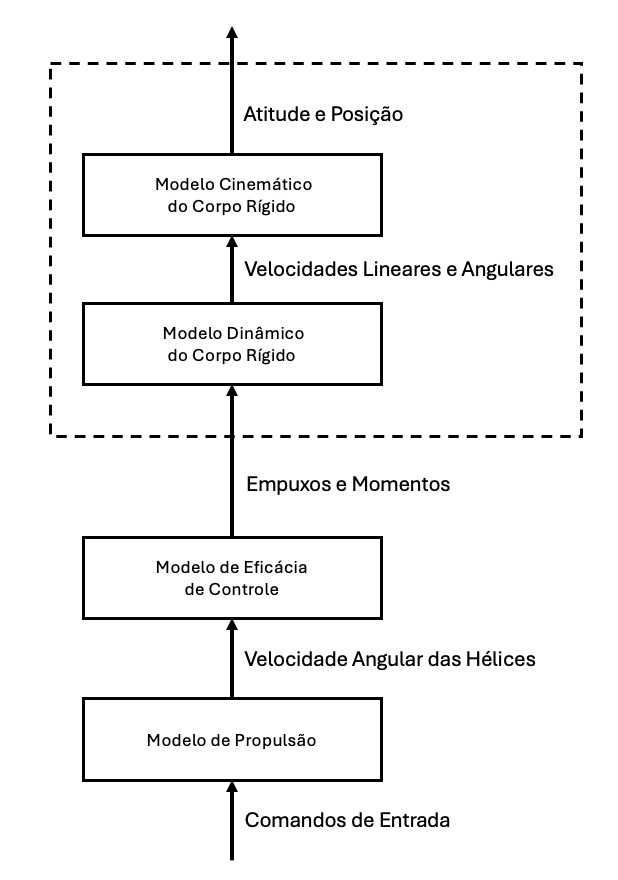
\includegraphics[width=0.4\textwidth]{Cap2/1.png}
  \caption{Submodelos do modo multirrotor (Adaptado de QUAN, 2017).}
  \label{motor-model}
\end{figure}

\subsection{Modelo de Propulsão do Motor}

A dinâmica do conjunto motor--ESC, também chamado de modelo de propulsão, que relaciona o comando de PWM $\sigma_i \in [0,1]$ à velocidade $\Omega_i$ com $i$ sendo a numeração dos motores, é bem aproximada por um sistema de primeira ordem \cite{Quan2017}. O comando de entrada impõe um valor de velocidade angular estacionário $\Omega_{ss,i}$, aplicado em um sistema de primeira ordem com constante de tempo $\tau_m$, resultando na relação entre o sinal de entrada e a velocidade angular do motor instantânea $\Omega_i$, dada por:
\begin{equation}
  \Omega_{ss,i}= C_R \sigma_i + \Omega_b
  \label{eq:motor-input}
\end{equation}

\begin{equation}
  \Omega_{i}= \frac{1}{\tau_m s + 1} \Omega_{ss,i}
  \label{eq:motor-input2}
\end{equation}

onde $C_R$ é uma constante de proporção, e $\Omega_b$ é a velocidade mínima inicial. A distribuição destas duas etapas pode ser vista na Figura \ref{motor} \cite{Quan2017}.

Cada um dos quatro motores \textit{brushless} rotaciona uma hélice que, ao girar com velocidade angular $\Omega_i$ produz um empuxo $T_i$ e um torque de reação $Q_i$, ambos proporcionais ao quadrado dessa velocidade angular, conforme a equação \ref{eq:motor-thrust} e \ref{eq:motor-torque} \cite{Graesdal2021,Quan2017,Cortez2022}:
\begin{equation}
    T_i = {c_T}_i\,\Omega_i^{2}
    \label{eq:motor-thrust}
\end{equation}
\begin{equation}
  Q_i = {c_M}_i\,\Omega_i^{2}
  \label{eq:motor-torque}
\end{equation}
em que ${c_T}_i$ e ${c_M}_i$ são os coeficientes de empuxo e de torque de cada motor, dependentes da geometria da hélice e da densidade do ar, obtidos experimentalmente em ensaios de bancada, conforme descrito no Apêndice~\ref{ap:bancada}.

Cabe ressaltar que os modelos das Equações \eqref{eq:motor-input} a \eqref{eq:motor-torque} estão ancorados na premissa de que a bateria se comporta como uma fonte de tensão ideal. Assume-se que a tensão de alimentação não sofre influências ambientais, como temperatura e pressão, nem varia com o estado de carga (\textit{State of Charge}, SOC) ou com o envelhecimento da sua química. Na prática, a queda de tensão ao longo do voo reduz a velocidade estacionária alcançada para um mesmo comando, efeito que se refletiria diretamente na constante $C_R$ da Equação \eqref{eq:motor-input}. Os parâmetros levantados neste trabalho representam, portanto, valores válidos para a condição de carga dos ensaios realizados.

\begin{figure}[ht]
  \centering
  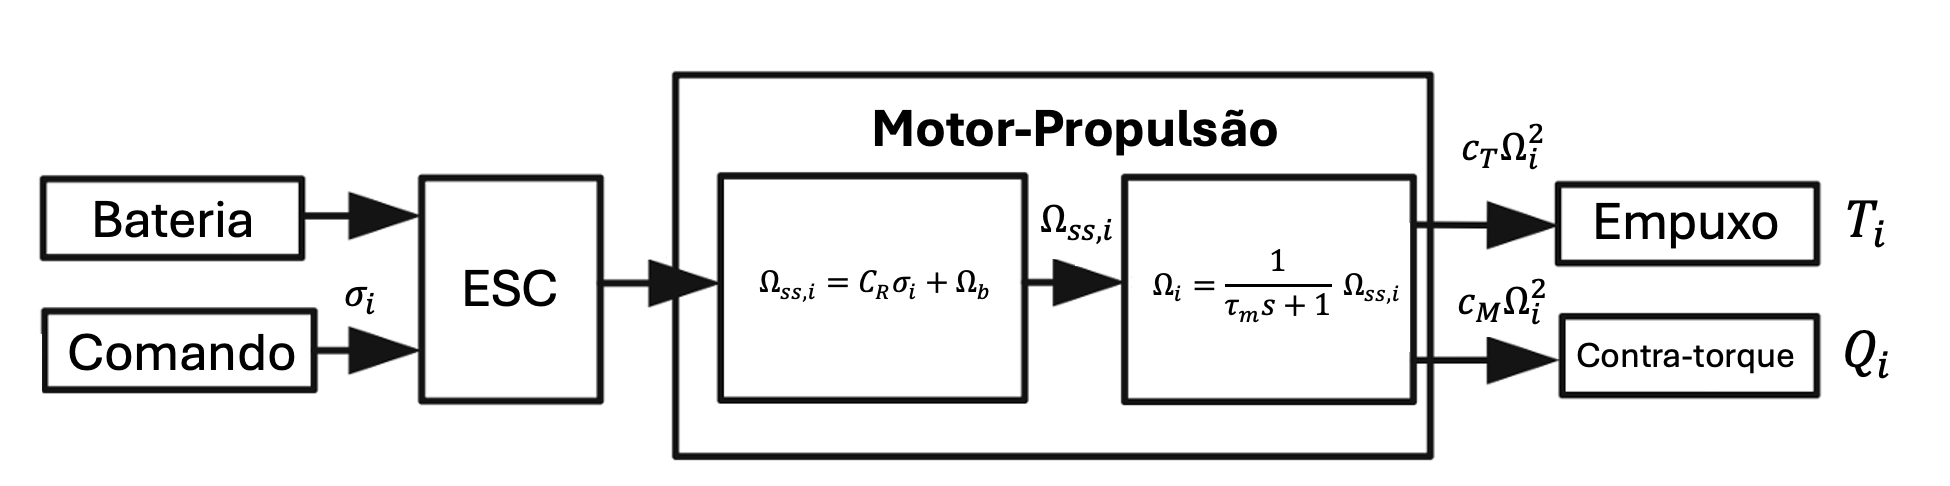
\includegraphics[width=0.9\textwidth]{Cap2/2.png}
  \caption{Modelo de motor brushless (Adaptado de QUAN, 2017).}
  \label{motor}
\end{figure}

\subsection{Alocação dos Motores}

Os empuxos individuais $T_i$ e os torques de reação $Q_i$ produzidos pelos quatro rotores combinam-se para gerar os esforços generalizados que atuam sobre o corpo da aeronave, como o empuxo total $T$, na direção do eixo $k^b$ do referencial do corpo \cite{Graesdal2021}.

\begin{equation}
  T = \sum_{i=1}^{4} T_i,
  \label{eq:thrust-total}
\end{equation}

A validade da Equação \eqref{eq:thrust-total} não depende da atitude da aeronave. Por ser escrita no referencial do corpo, com os eixos dos quatro rotores paralelos a $k^b$, a soma dos empuxos individuais representa o esforço resultante para quaisquer ângulos de rolagem e arfagem, cujo efeito é tratado pela projeção da gravidade nas equações translacionais, conforme a Equação \eqref{eq:w_dot}. 

As condições de contorno da equação são: a montagem dos rotores deve permanecer rígida e paralela entre si, os coeficientes ${c_T}_i$ e ${c_M}_i$, levantados em bancada estática, valem para o voo pairado e baixas velocidades, e desprezam-se as interferências aerodinâmicas entre rotores e com a asa fixa, além do efeito solo. Essas restrições são compatíveis com o recorte deste trabalho, concentrado no modo multirrotor em torno do voo pairado.

Os momentos gerados pelos rotores compõem o vetor $\boldsymbol{\tau}^{b} = [\tau_x\ \ \tau_y\ \ \tau_z]^{\top}$, expresso no referencial do corpo e obtido pela soma dos produtos vetoriais entre a posição $\mathbf{r}_i$ de cada rotor em relação ao CG e o respectivo empuxo $\mathbf{T}_i = -T_i\,\mathbf{k}^b$, acrescida dos torques de reação $\mathbf{Q}_i$, alinhados a $\mathbf{k}^b$ \cite{Beard2012}:

\begin{equation}
  \boldsymbol{\tau}^{b} = \sum_{i=1}^{4} \mathbf{r}_i \times \mathbf{T}_i + \sum_{i=1}^{4} \mathbf{Q}_i.
  \label{eq:tau-vetorial}
\end{equation}

Como os empuxos são paralelos a $k^b$, o produto vetorial de cada rotor produz componentes apenas nos eixos $i^b$ e $j^b$, proporcionais ao empuxo e aos braços horizontais em relação ao CG. Dessa forma, o empuxo não contribui para a guinada, que decorre apenas dos torques de reação, e a posição vertical dos rotores não afeta os momentos. As Equações \eqref{eq:tau_x} a \eqref{eq:tau_z} apresentam as componentes escalares desse vetor em cada eixo, conforme ilustra a Figura~\ref{force-moment}, e é nessa forma vetorial que os momentos entram no modelo rotacional da Equação \eqref{eq:second-law-rotation}.

\begin{align}
  \tau_x &= -\sum_{i=1}^{4} L_{i,y}\,T_i, \label{eq:tau_x} \\[2pt]
  \tau_y &= \phantom{-}\sum_{i=1}^{4} L_{i,x}\,T_i, \label{eq:tau_y} \\[2pt]
  \tau_z &= Q_1 + Q_2 - Q_3 - Q_4 \label{eq:tau_z}
\end{align}

Diferentemente de um quadrirrotor simétrico, em que todos os rotores se encontram a uma mesma distância $L$ do centro de gravidade, o drone VTOL híbrido deste trabalho admite valores distintos, portanto, definem-se as distâncias do centro de gravidade até cada rotor como sendo: 

\begin{itemize}
  \item $L_{x_r}$ e $L_{x_l}$ são as distâncias laterais aos rotores dos lados direito e esquerdo;
  \item $L_{y_f}$ e $L_{y_r}$, as distâncias longitudinais aos rotores dianteiros e traseiros. 
\end{itemize}

Com isso obtém-se a soma das influências de cada motor no esforço agregado de forças e momentos sobre o corpo rígido do VTOL \cite{Quan2017}:

\begin{equation}
    \begin{bmatrix} T \\ \tau_x \\ \tau_y \\ \tau_z \end{bmatrix}
    =
    \begin{bmatrix}
        1        & 1        & 1        & 1        \\
        -L_{x_r} & L_{x_l}  & L_{x_l}  & -L_{x_r} \\
        L_{y_f}  & -L_{y_r} & L_{y_f}  & -L_{y_r} \\
        0        & 0        & 0        & 0
    \end{bmatrix}
    \begin{bmatrix} T_1 \\ T_2 \\ T_3 \\ T_4 \end{bmatrix}
    +
    \begin{bmatrix}
        0 & 0 & 0 & 0 \\
        0 & 0 & 0 & 0 \\
        0 & 0 & 0 & 0 \\
        1 & 1 & -1 & -1
    \end{bmatrix}
    \begin{bmatrix} Q_1 \\ Q_2 \\ Q_3 \\ Q_4 \end{bmatrix}
    \label{eq:alocacao-detalhe}
\end{equation}

A partir do modelo do motor-propulsão, definido nas Equações \eqref{eq:motor-thrust} e \eqref{eq:motor-torque}, pode-se obter a relação entre o torque de reação e o empuxo de cada rotor, com a razão entre os coeficientes admitida comum aos quatro rotores:

\begin{equation}
  Q_i = \frac{c_M}{c_T}\,T_i,
  \label{eq:razao-QT}
\end{equation}

o que permite expressar o momento de guinada diretamente em função dos empuxos. Com isso, as duas parcelas da Equação~\eqref{eq:alocacao-detalhe} reduzem-se a uma única matriz $\mathbf{B}$, também denominada matriz de alocação, que mapeia os empuxos dos rotores nos esforços generalizados:
\begin{equation}
    \begin{bmatrix} T \\ \tau_x \\ \tau_y \\ \tau_z \end{bmatrix} =
    \underbrace{\begin{bmatrix}
        1                & 1                & 1                 & 1                 \\
        -L_{x_r}         & L_{x_l}          & L_{x_l}           & -L_{x_r}          \\
        L_{y_f}          & -L_{y_r}         & L_{y_f}           & -L_{y_r}          \\
        \dfrac{c_M}{c_T} & \dfrac{c_M}{c_T} & -\dfrac{c_M}{c_T} & -\dfrac{c_M}{c_T}
    \end{bmatrix}}_{\mathbf{B}}
    \begin{bmatrix} T_1 \\ T_2 \\ T_3 \\ T_4 \end{bmatrix}
    \label{eq:alocacao}
\end{equation}

Para o quadrirrotor, a matriz $\mathbf{B}$ é quadrada e inversível, o que permite resolver o problema de alocação de controle: dado o esforço desejado $\mathbf{u} = [\,T\ \ \tau_x\ \ \tau_y\ \ \tau_z\,]^{\mathsf{T}}$, os empuxos que cada rotor deve produzir são obtidos por $[\,T_1\ \ T_2\ \ T_3\ \ T_4\,]^{\mathsf{T}} = \mathbf{B}^{-1}\,\mathbf{u}$ e, por meio do modelo do motor da Equação~\eqref{eq:motor-thrust}, \eqref{eq:motor-torque} e \eqref{eq:motor-input}, obtém-se as respectivas velocidades $\Omega_i$ e os comandos $\sigma_i$.

\subsection{Modelo Rotacional}

A elaboração do modelo rotacional é detalhado por \textcite{Beard2012}, onde esta é derivada da segunda lei de newton que determina:

\begin{equation}
  \frac{d \mathbf{h}}{dt} = \boldsymbol{\tau},
  \label{eq:second-law-rotation}
\end{equation}

onde $\mathbf{h}$ é o momento angular, e $\boldsymbol{\tau}$ é a soma de todos os momentos aplicados ao corpo rígido do drone híbrido. A transformação da representação do sistema inercial para o sistema corpo resulta em:

\begin{equation}
  \frac{d \mathbf{h}}{dt} = \frac{d \mathbf{h^b}}{dt} + \boldsymbol{\omega_b} \times \mathbf{h^b}= \boldsymbol{\tau^b},
  \label{eq:second-law-rotation1}
\end{equation}
\begin{equation}
  \mathbf{h^b}=\mathbf{J} \boldsymbol{\omega_b},
  \label{eq:second-law-rotation2}
\end{equation}

lembrando que $\boldsymbol{\dot{\omega_b}} = [\dot{p},\dot{q},\dot{r}]^T$, representnado as acelerações angulares, onde $\mathbf{J}$, apresentado na Equação \eqref{eq:matrizinercia}, é a matriz dos momentos de inércia do corpo rígido. Este corpo não é simétrico em relação ao eixo $j^b$ \cite{Beard2012, Graesdal2021}, portanto, difere das formulações de MAVs multirrotores que possuem apenas matriz diagonal, devido a sua estrutura de asa fixa, algo que impacta diretamente no resultado da formulação do modelo rotacional e difere das abordagens convencionais de multirrotor \cite{Bouabdallah2007,Carino2015}.

\begin{equation}
  \mathbf{J}
  =
  \begin{bmatrix}
      J_{xx} & 0 & -J_{xz} \\
      0 & J_{yy} & 0 \\
      -J_{xz} & 0 & J_{zz} \\
  \end{bmatrix}
  \label{eq:matrizinercia}
\end{equation}

Considerando a presença de um arrasto angular, representados pelos coeficientes de arrasto $c_p$, $c_q$ e $c_r$, proporcionais às velocidades angulares, conforme ilustrado por \textcite{Quan2017} na Figura \ref{arrasto1}, o escoamento incidente nas hélices gera uma força de arrasto que, atuando a uma distância do centro de gravidade, produz um torque de arrasto. Quando esse escoamento é induzido pela própria rotação do corpo, com cada rotor deslocando-se a uma velocidade proporcional à taxa angular e ao braço, o torque resultante opõe-se ao giro, dando origem aos termos de amortecimento adotados no modelo rotacional.

Além disso o torque gerados pelos motores $\boldsymbol{\tau^b}=[\tau_x, \tau_y, \tau_z]$ das Equação \eqref{eq:alocacao}, é possível formular o modelo rotacional substituindo a Equação \eqref{eq:second-law-rotation2} em \eqref{eq:second-law-rotation1}, obtém-se:

\begin{equation}
  \frac{d \mathbf{\boldsymbol{\omega_b}}}{dt} = \mathbf{J^{-1}}[-\boldsymbol{\omega_b} \times (\mathbf{J} \boldsymbol{\omega_b})+\boldsymbol{\tau^b}]
  \label{eq:second-law-rotation3}
\end{equation}

\begin{equation}
  \begin{bmatrix} \dot{p} \\ \dot{q} \\ \dot{r} \end{bmatrix}
  = \mathbf{J}^{-1}\left[
  -\begin{bmatrix} 0 & -r & q \\ r & 0 & -p \\ -q & p & 0 \end{bmatrix}
  \begin{bmatrix} J_{xx} & 0 & -J_{xz} \\ 0 & J_{yy} & 0 \\ -J_{xz} & 0 & J_{zz} \end{bmatrix}
  \begin{bmatrix} p \\ q \\ r \end{bmatrix}
  + \begin{bmatrix} \tau_x \\ \tau_y \\ \tau_z \end{bmatrix}
  \right]
  \label{eq:rot-matricial}
  \end{equation}

\begin{figure}[ht]
  \centering
  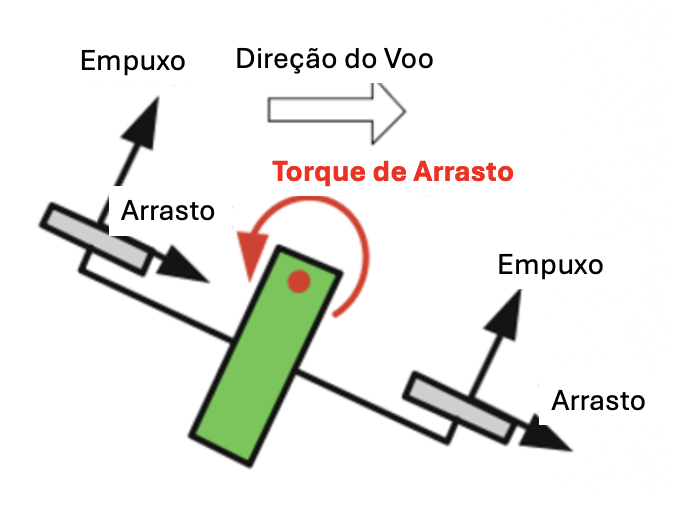
\includegraphics[width=0.4\textwidth]{Cap2/drag.png}
  \caption{Arrasto proporcional a velocidade angular \cite[Adaptado de][]{Beard2012}.}
  \label{arrasto1}
\end{figure}

A dinâmica rotacional do corpo rígido, assumindo que o VTOL está em modo quadrirrotor, com uma velocidade longitudinal desprezível, reduzindo, portanto, os momentos de arrasto aerodinâmicos da estrutura de asa-fixa, é descrita pelas equações: 

\begin{align}
  \dot{p} &= \Gamma_1\,pq - \Gamma_2\,qr + \Gamma_3\,\tau_x + \Gamma_4\,\tau_z - c_p p, \label{eq:p_dot} \\
  \dot{q} &= \Gamma_5\,pr - \Gamma_6\,(p^2 - r^2) + \frac{1}{J_y}\,\tau_y - c_q q, \label{eq:q_dot} \\
  \dot{r} &= \Gamma_7\,pq - \Gamma_1\,qr + \Gamma_4\,\tau_x + \Gamma_8\,\tau_z - c_r r. \label{eq:r_dot}
\end{align}

em que os coeficientes $\Gamma_i$ agrupam os termos de inércia, com $\Gamma = J_x J_z - J_{xz}^2$:
\begin{equation}
\begin{aligned}
    \Gamma_1 &= \frac{J_{xz}(J_x - J_y + J_z)}{\Gamma}, &
    \Gamma_2 &= \frac{J_z(J_z - J_y) + J_{xz}^2}{\Gamma}, \\
    \Gamma_3 &= \frac{J_z}{\Gamma}, &
    \Gamma_4 &= \frac{J_{xz}}{\Gamma}, \\
    \Gamma_5 &= \frac{J_z - J_x}{J_y}, &
    \Gamma_6 &= \frac{J_{xz}}{J_y}, \\
    \Gamma_7 &= \frac{(J_x - J_y)J_x + J_{xz}^2}{\Gamma}, &
    \Gamma_8 &= \frac{J_x}{\Gamma}.
\end{aligned}
\label{eq:gammas}
\end{equation}

\subsection{Modelo Translacional}

O modelo translacional do drone híbrido é determinado pela segunda lei de Newton aplicada ao corpo rígido, conforme a equação \eqref{eq:second-law-translational}. Neste trabalho, a dedução do modelo foi baseada em \textcite{Beard2012}, adaptado para VTOL por \textcite{Graesdal2021}. Da segunda lei de Newton:

\begin{equation}
  m\frac{d \mathbf{v}}{dt} = \mathbf{f},
  \label{eq:second-law-translational}
\end{equation}
onde $\mathbf{m}$ é a massa, $\mathbf{v}$ é a velocidade linear e $\mathbf{f}$ é a soma de todas as forças aplicadas ao corpo do drone híbrido. Assim como no modelo rotacional é feita a transformação da representação desse termo do sistema inercial para o corpo, que resulta em:

\begin{equation}
  m \frac{d \mathbf{v}}{dt} = m \left( \frac{d \mathbf{v^b}}{dt} + \boldsymbol{\omega_b} \times \mathbf{v^b} \right) = \mathbf{f^b},
  \label{eq:second-law-translational1}
\end{equation}
levando em consideração que $\dot{\mathbf{v}^b}=[\dot{u}, \dot{v}, \dot{w}]^T$, tem-se que a únicas forças aplicadas no mulitirrotor é o empuxo total gerado pelos motores $T$ no eixo $k^b$, e a força da gravidade transformada para o sistema de referecial do corpo, definido pela Equação \eqref{eq:g-corpo}, portanto:

\begin{equation}
  \mathbf{f^b} = \begin{bmatrix} 0 \\ 0 \\ -T \end{bmatrix} + \begin{bmatrix} -\,g\,s_\theta \\ g\,s_\phi c_\theta \\ g\,c_\phi c_\theta \end{bmatrix}
  \label{eq:second-law-translational2}
\end{equation}

Substituindo a equação \eqref{eq:second-law-rotation2} em\eqref{eq:second-law-rotation1}, obtem-se:

\begin{equation}
  \begin{bmatrix} \dot{u} \\ \dot{v} \\ \dot{w} \end{bmatrix}
  = -\begin{bmatrix} 0 & -r & q \\ r & 0 & -p \\ -q & p & 0 \end{bmatrix}
  \begin{bmatrix} u \\ v \\ w \end{bmatrix}
  + \frac{1}{m}\begin{bmatrix} 0 \\ 0 \\ -T \end{bmatrix}
  + \begin{bmatrix} -g\,s_\theta \\ g\,s_\phi c_\theta \\ g\,c_\phi c_\theta \end{bmatrix}
  \label{eq:trans-matricial}
  \end{equation}

Utilizando a Equação \eqref{eq:second-law-translational1}, assumindo que a velocidade longitudinal é desprezível, retirando a sustentação e arrastos decorrentes da estrutura de asa fixa, é possível obter as equações que regem o modelo translacional do drone híbrido:

\begin{align}
  \dot{u} &= rv - qw - g\,s_\theta, \label{eq:u_dot} \\
  \dot{v} &= pw - ru + g\,s_\phi c_\theta, \label{eq:v_dot} \\
  \dot{w} &= qu - pv - \frac{T}{m} + g\,c_\phi c_\theta. \label{eq:w_dot}
\end{align}

\subsection{Compensações e correções nas leituras de acelerômetros}

Diferentemente das equações de movimento, que descrevem a dinâmica do corpo rígido no centro de massa, a resposta do acelerômetro é uma equação de saída, que relaciona os estados às grandezas efetivamente lidas pelo sensor. 

O acelerômetro, integrado à unidade de medição inercial (IMU), não mede a aceleração do centro de massa, mas sim a força específica. Trata-se da resultante, por unidade de massa, das forças de contato aplicadas ao corpo, $\mathbf{f} = \mathbf{a} - \mathbf{g}^{b}$, pois somente essas forças produzem a deflexão relativa entre a carcaça e a massa de prova que o sensor transduz. A leitura é realizada no ponto em que o sensor está montado. Como esse ponto está deslocado do centro de massa por um vetor $\mathbf{r}_{imu} = [\,r_x\ \ r_y\ \ r_z\,]^{\mathsf{T}}$, expresso no referencial do corpo, a leitura incorpora um efeito de braço de alavanca \cite{Farrell2008}.

\begin{figure}[ht]
  \centering
  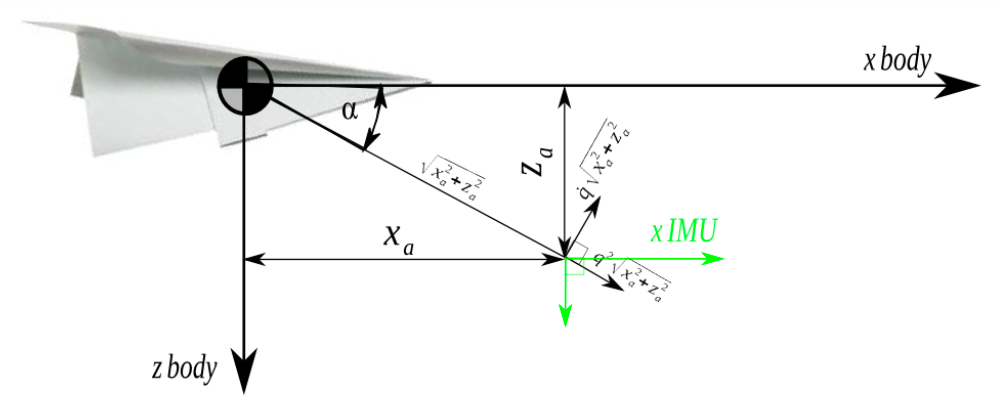
\includegraphics[width=0.6\textwidth]{Cap2/ACELEROMETER.png}
  \caption{Deslocamento do acelerômetro do CG.}
  \label{acelerometer-displacement}
\end{figure}


Transportando essa força específica do centro de massa para a posição do sensor, somam-se um termo tangencial (devido à aceleração angular) e um termo centrípeto \cite{Tischler2012}:
\begin{equation}
    \mathbf{a}_{imu}^{b} = \mathbf{a}_{cg}^{b}
    + \underbrace{\dot{\boldsymbol{\omega}}^{b} \times \mathbf{r}_{imu}}_{\text{tangencial}}
    + \underbrace{\boldsymbol{\omega}^{b} \times \left(\boldsymbol{\omega}^{b} \times \mathbf{r}_{imu}\right)}_{\text{centrípeto}}
    + \mathbf{b},
    \label{eq:acc-imu}
\end{equation}
em que $\boldsymbol{\omega}^{b} = [\,p\ \ q\ \ r\,]^{\mathsf{T}}$, $\dot{\boldsymbol{\omega}}^{b} = [\,\dot p\ \ \dot q\ \ \dot r\,]^{\mathsf{T}}$. Sendo $\mathbf{b} = [\,b_x\ \ b_y\ \ b_z\,]^{\mathsf{T}}$ o viés (\textit{bias}) constante do sensor, uma propriedade do hardware. Expandindo os produtos vetoriais, as três componentes da força específica medida resultam em:
\begin{align}
    a_x &= (\dot q\, r_z - \dot r\, r_y) + p q\, r_y + p r\, r_z - (q^2 + r^2)\, r_x + b_x, \label{eq:acc-x} \\
    a_y &= (\dot r\, r_x - \dot p\, r_z) + p q\, r_x + q r\, r_z - (p^2 + r^2)\, r_y + b_y, \label{eq:acc-y} \\
    a_z &= -\frac{T}{m} + (\dot p\, r_y - \dot q\, r_x) + p r\, r_x + q r\, r_y - (p^2 + q^2)\, r_z + b_z. \label{eq:acc-z}
\end{align}

Observa-se que, em razão do deslocamento $\mathbf{r}_{imu}$, as acelerações angulares $\dot p$, $\dot q$ e $\dot r$ e as velocidades angulares $p$, $q$ e $r$ acoplam-se diretamente na medida do acelerômetro. Esse acoplamento é particularmente relevante para a identificação, pois faz com que o sinal do acelerômetro carregue informação sobre a dinâmica rotacional, sendo considerado na estimação dos parâmetros.

\subsection{Equação Cinemática de Euler}

A relação entre as velocidades angulares no referencial do corpo ($p$, $q$, $r$) e as taxas de variação dos ângulos de Euler ($\dot\phi$, $\dot\theta$, $\dot\psi$) é dada pela matriz de transformação cinemática \cite{Farrell2008}:
\begin{equation}
  \begin{bmatrix} \dot{\phi} \\ \dot{\theta} \\ \dot{\psi} \end{bmatrix}
  =
  \begin{bmatrix}
      1 & s_\phi\,t_\theta & c_\phi\,t_\theta \\[2pt]
      0 & c_\phi & -s_\phi \\[2pt]
      0 & s_\phi/c_\theta & c_\phi/c_\theta
  \end{bmatrix}
  \begin{bmatrix} p \\ q \\ r \end{bmatrix}.
  \label{eq:euler-kinematic}
\end{equation}

Essa transformação é necessária porque as velocidades angulares $p$, $q$ e $r$ estão expressas no referencial do corpo, enquanto a atitude da aeronave é descrita pelos ângulos de Euler, definidos em relação ao referencial de navegação. Como os ângulos de Euler resultam de rotações sucessivas em torno de eixos distintos, suas taxas de variação $\dot\phi$, $\dot\theta$ e $\dot\psi$ não correspondem diretamente às componentes da velocidade angular do corpo.

Observa-se ainda que essa parametrização apresenta uma singularidade em $\theta = \pm 90^\circ$, na qual $c_\theta = 0$ e a terceira linha da matriz diverge; tal condição, contudo, está fora do envelope de voo em modo multirrotor considerado neste trabalho.

\subsection{Modelo não linear}

Qualquer plataforma aérea com estrutura física semelhante à do drone híbrido deste trabalho, ilustrada na Figura~\ref{force-moment}, operando em modo quadrirrotor, pode ser representada pelo conjunto de equações não lineares deduzido neste capítulo. O modelo reúne a cinemática de atitude, a dinâmica rotacional e a dinâmica translacional do corpo rígido, alimentadas pelos esforços generalizados gerados pelos motores. As equações são reapresentadas a seguir com a sua numeração original, para consolidar o modelo completo.

A geração desses esforços parte do modelo de propulsão, em que cada comando $\sigma_i$ define a velocidade angular do rotor e, desta, o empuxo e o torque de reação
\begin{equation*}
  \Omega_{ss,i} = C_R\,\sigma_i + \Omega_b
  \qquad
  \Omega_i = \frac{1}{\tau_m s + 1}\,\Omega_{ss,i}
  \tag{\ref{eq:motor-input}, \ref{eq:motor-input2}}
\end{equation*}
\begin{equation*}
  T_i = {c_T}_i\,\Omega_i^{2}
  \qquad
  Q_i = {c_M}_i\,\Omega_i^{2}
  \tag{\ref{eq:motor-thrust}, \ref{eq:motor-torque}}
\end{equation*}
que a matriz de alocação combina no empuxo total e nos momentos de controle
\begin{equation*}
    \begin{bmatrix} T \\ \tau_x \\ \tau_y \\ \tau_z \end{bmatrix} =
    \begin{bmatrix}
        1 & 1 & 1 & 1 \\
        -L_{x_r} & L_{x_l} & L_{x_l} & -L_{x_r} \\
        L_{y_f} & -L_{y_r} & L_{y_f} & -L_{y_r} \\
        \dfrac{c_M}{c_T} & \dfrac{c_M}{c_T} & -\dfrac{c_M}{c_T} & -\dfrac{c_M}{c_T}
    \end{bmatrix}
    \begin{bmatrix} T_1 \\ T_2 \\ T_3 \\ T_4 \end{bmatrix}
    \tag{\ref{eq:alocacao}}
\end{equation*}

Com o empuxo total $T$ e os momentos $\tau_x$, $\tau_y$ e $\tau_z$ assim definidos, a dinâmica do corpo rígido em modo quadrirrotor é descrita pelas nove equações de estado a seguir.

A cinemática de atitude relaciona as velocidades angulares do corpo às taxas dos ângulos de Euler
\begin{equation*}
\begin{aligned}
  \dot{\phi} &= p + s_\phi t_\theta\,q + c_\phi t_\theta\,r \\
  \dot{\theta} &= c_\phi\,q - s_\phi\,r \\
  \dot{\psi} &= \frac{s_\phi}{c_\theta}\,q + \frac{c_\phi}{c_\theta}\,r
\end{aligned}
\tag{\ref{eq:euler-kinematic}}
\end{equation*}

A dinâmica rotacional é governada pelo tensor de inércia e pelos arrastos angulares
\begin{align*}
  \dot{p} &= \Gamma_1\,pq - \Gamma_2\,qr + \Gamma_3\,\tau_x + \Gamma_4\,\tau_z - c_p\,p \tag{\ref{eq:p_dot}} \\
  \dot{q} &= \Gamma_5\,pr - \Gamma_6\,(p^2 - r^2) + \frac{1}{J_y}\,\tau_y - c_q\,q \tag{\ref{eq:q_dot}} \\
  \dot{r} &= \Gamma_7\,pq - \Gamma_1\,qr + \Gamma_4\,\tau_x + \Gamma_8\,\tau_z - c_r\,r \tag{\ref{eq:r_dot}}
\end{align*}

A dinâmica translacional reúne os termos de Coriolis, a gravidade projetada no referencial do corpo e o empuxo no eixo $k^b$
\begin{align*}
  \dot{u} &= rv - qw - g\,s_\theta \tag{\ref{eq:u_dot}} \\
  \dot{v} &= pw - ru + g\,s_\phi c_\theta \tag{\ref{eq:v_dot}} \\
  \dot{w} &= qu - pv - \frac{T}{m} + g\,c_\phi c_\theta \tag{\ref{eq:w_dot}}
\end{align*}

O caráter não linear do modelo reside em dois tipos de termo dessas equações. O primeiro são os produtos entre estados, como $pq$ e $qr$ nos termos giroscópicos da dinâmica rotacional e $rv$ e $qu$ nos termos de Coriolis da translacional, que violam o princípio da superposição. O segundo são as funções trigonométricas dos estados de atitude, presentes na cinemática de Euler e na projeção da gravidade sobre o corpo. Soma-se a eles, na cadeia de atuação, a dependência quadrática do empuxo e do torque com a velocidade de cada rotor, conforme as Equações \eqref{eq:motor-thrust} e \eqref{eq:motor-torque}. As entradas generalizadas $T$, $\tau_x$, $\tau_y$ e $\tau_z$, por outro lado, entram linearmente nas equações de estado, propriedade que torna a matriz de entrada constante na linearização apresentada no Apêndice~\ref{ap:linearizacao}, na qual os produtos entre estados se anulam no equilíbrio e as funções trigonométricas se reduzem aos próprios ângulos.

Identificar a aeronave consiste em determinar os valores numéricos dos parâmetros deste modelo de modo que o conjunto de equações, com os parâmetros identificados, reproduza o comportamento observado nos ensaios em voo, tarefa desenvolvida no próximo capítulo.
